\documentclass[12pt]{article}
\usepackage[utf8]{inputenc}
\usepackage[utf8]{inputenc}
\usepackage{amsmath}
\usepackage{amsthm}
\usepackage{amssymb}
\usepackage{array}
\usepackage{geometry}
\usepackage{amsfonts}
\usepackage{mathrsfs}
\usepackage{bm}
\usepackage{hyperref}
\usepackage{float}
\usepackage[dvipsnames]{xcolor}
\usepackage[inline]{enumitem}
\usepackage{mathtools}
\usepackage{changepage}
\usepackage{graphicx}
\usepackage{systeme}
\usepackage{caption}
\usepackage{subcaption}
\usepackage[breakable]{tcolorbox}
\usepackage[linguistics]{forest}
\usepackage{tikz}
\usetikzlibrary{matrix, patterns, decorations.pathreplacing, calligraphy}
\usepackage{tikz-cd}
\usepackage[nameinlink]{cleveref}
\geometry{
headheight=15pt,
left=60pt,
right=60pt
}
\setlength{\emergencystretch}{20pt}
\usepackage{fancyhdr}
\pagestyle{fancy}
\fancyhf{}
\lhead{}
\chead{Section 8.4 Exercises}
\rhead{\thepage}
\hypersetup{
    colorlinks=true,
    linkcolor=blue,
    urlcolor=blue
}

\theoremstyle{definition}
\newtheorem*{remark}{Remark}

\newtheoremstyle{exercise}
    {}
    {}
    {}
    {}
    {\bfseries}
    {.}
    { }
    {\thmname{#1}\thmnumber{#2}\thmnote{ (#3)}}
\theoremstyle{exercise}
\newtheorem{exercise}{Exercise 8.4.}

\newtheoremstyle{solution}
    {}
    {}
    {}
    {}
    {\itshape\color{magenta}}
    {.}
    { }
    {\thmname{#1}\thmnote{ #3}}
\theoremstyle{solution}
\newtheorem*{solution}{Solution}

\Crefformat{exercise}{#2Exercise 8.4.#1#3}

\tcbset{colback=blue!5!white}

\newcommand{\interior}[1]{%
  {\kern0pt#1}^{\mathrm{o}}%
}
\newcommand{\ts}{\textsuperscript}
\newcommand{\setcomp}[1]{#1^{\mathsf{c}}}
\newcommand{\poly}{\mathcal{P}}
\newcommand{\quand}{\quad \text{and} \quad}
\newcommand{\quimplies}{\quad \implies \quad}
\newcommand{\quiff}{\quad \iff \quad}
\newcommand{\N}{\mathbf{N}}
\newcommand{\Z}{\mathbf{Z}}
\newcommand{\Q}{\mathbf{Q}}
\newcommand{\I}{\mathbf{I}}
\newcommand{\R}{\mathbf{R}}
\newcommand{\C}{\mathbf{C}}

\DeclarePairedDelimiter\abs{\lvert}{\rvert}
% Swap the definition of \abs* and \norm*, so that \abs
% and \norm resizes the size of the brackets, and the 
% starred version does not.
\makeatletter
\let\oldabs\abs
\def\abs{\@ifstar{\oldabs}{\oldabs*}}

\DeclarePairedDelimiter\norm{\lVert}{\rVert}
\makeatletter
\let\oldnorm\norm
\def\norm{\@ifstar{\oldnorm}{\oldnorm*}}
\makeatother

\DeclarePairedDelimiter\paren{(}{)}
\makeatletter
\let\oldparen\paren
\def\paren{\@ifstar{\oldparen}{\oldparen*}}
\makeatother

\DeclarePairedDelimiter\bkt{[}{]}
\makeatletter
\let\oldbkt\bkt
\def\bkt{\@ifstar{\oldbkt}{\oldbkt*}}
\makeatother

\DeclarePairedDelimiter\set{\{}{\}}
\makeatletter
\let\oldset\set
\def\set{\@ifstar{\oldset}{\oldset*}}
\makeatother

\setlist[enumerate,1]{label={(\alph*)}}

\begin{document}

\section{Section 8.4 Exercises}

Exercises with solutions from Section 8.4 of \hyperlink{ua}{[UA]}.

\begin{exercise}
\label{ex:1}
    For \( n \in \N \), let
    \[
        n\# = n + (n - 1) + (n - 2) + \cdots + 2 + 1.
    \]
    \begin{enumerate}
        \item Without looking ahead, decide if there is a natural way to define \( 0\# \). How about \( (-2)\# \)? Conjecture a reasonable value for \( \tfrac{7}{2} \# \).

        \item Now prove \( n\# = \tfrac{1}{2} n(n + 1) \) for all \( n \in \N \), and revisit part (a).
    \end{enumerate}
\end{exercise}

\begin{solution}
    \begin{enumerate}
        \item We observe that \( n\# \) satisfies the relation \( n\# = n + (n - 1)\# \) for \( n \geq 2 \); it seems reasonable to use this relation to extend the definition of \( \# \). Thus
        \[
            1\# = 1 + 0\# \quimplies 0\# = 1 - 1\# = 0.
        \]
        Similarly,
        \[
            0\# = (-1)\# = -1 + (-2)\# \quimplies (-2)\# = 1.
        \]
        Some more calculations show that
        \[
            1\# + (-1)\# = 1, \quad 2\# + (-2)\# = 4, \quand 3\# + (-3)\# = 9.
        \]
        Given this, we might conjecture that \( n\# + (-n)\# = n^2 \) for \( n \in \N \). Using this identity and the previous recurrence relation, we find that \( \tfrac{1}{2} \# = \tfrac{1}{2} + \paren{ -\tfrac{1}{2} } \# = \tfrac{3}{8} \) and thus
        \[
            \frac{7}{2} \# = \frac{15}{2} + \frac{1}{2} \# = \frac{63}{8}.
        \]

        \item This is a \href{https://en.wikipedia.org/wiki/Mathematical_induction#Sum_of_consecutive_natural_numbers}{classic result}, the proof of which is likely one of the first encountered by students learning mathematical induction, and so I won't repeat it here. \href{https://nrich.maths.org/2478}{Another method, perhaps more satisfying, is often attributed to Gauss} (whether this story is true or not is \href{https://hsm.stackexchange.com/questions/384/did-gauss-find-the-formula-for-123-ldotsn-2n-1n-in-elementary-school}{unclear}; he certainly wouldn't have been the first to find this formula).

        Taking \( n = 0, -2, \) and \( \tfrac{7}{2} \) in this formula confirms our conjectures from part (a).
    \end{enumerate}
\end{solution}

\begin{exercise}
\label{ex:2}
    Verify that the series converges absolutely for all \( x \in \R \), that \( E(x) \) is differentiable on \( \R \), and \( E'(x) = E(x) \).
\end{exercise}

\begin{solution}
    For a given non-zero \( x \in \R \), note that
    \[
        \frac{\abs{x}^{n+1}}{(n + 1)!} \cdot \frac{n!}{\abs{x}^n} = \frac{\abs{x}}{n + 1} \to 0;
    \]
    it follows from the Ratio Test (\href{https://lew98.github.io/Mathematics/UA_Section_2_7_Exercises.pdf}{Exercise 2.7.9}) that the series \( \sum_{n=0}^{\infty} \tfrac{x^n}{n!} \) converges absolutely. Theorem 6.5.7 now implies that \( E \) is differentiable on \( \R \) and furthermore that
    \[
        E'(x) = \sum_{n=1}^{\infty} \frac{n x^{n-1}}{n!} = \sum_{n=1}^{\infty} \frac{x^{n-1}}{(n - 1)!} = \sum_{n=0}^{\infty} \frac{x^n}{n!} = E(x).
    \]
\end{solution}

\begin{exercise}
\label{ex:3}
    \begin{enumerate}
        \item Use the results of \href{https://lew98.github.io/Mathematics/UA_Section_2_8_Exercises.pdf}{Exercise 2.8.7} and the binomial formula to show that \( E(x + y) = E(x) E(y) \) for all \( x, y \in \R \).

        \item Show that \( E(0) = 1, E(-x) = 1 / E(x), \) and \( E(x) > 0 \) for all \( x \in \R \).
    \end{enumerate}
\end{exercise}

\begin{solution}
    \begin{enumerate}
        \item Let \( x, y \in \R \) be given and for each \( n \geq 0 \) let \( a_n = \tfrac{y^n}{n!} \) and \( b_n = \tfrac{x^n}{n!} \). For each \( k \geq 0 \), define
        \[
            d_k = a_0 b_k + \cdots + a_k b_0 = \sum_{n=0}^k a_n b_{k-n} = \sum_{n=0}^k \frac{x^{k-n} y^n}{(k-n)! n!} = \frac{1}{k!} \sum_{n=0}^k \binom{k}{n} x^{k-n} y^n = \frac{(x + y)^k}{k!}.
        \]
        It follows that for each \( N \geq 0 \) we have
        \[
            \sum_{k=0}^N d_k = \sum_{k=0}^N \frac{(x + y)^k}{k!}.
        \]
        On one hand, \( \sum_{k=0}^N \frac{(x + y)^k}{k!} \to E(x + y) \) as \( N \to \infty \); on the other hand,
        \[
            \sum_{k=0}^N d_k \to \paren{ \sum_{n=0}^{\infty} b_n } \paren{ \sum_{n=0}^{\infty} a_n } = E(x) E(y) \text{ as } N \to \infty
        \]
        by \href{https://lew98.github.io/Mathematics/UA_Section_2_8_Exercises.pdf}{Exercise 2.8.7}. We may conclude that \( E(x + y) = E(x) E(y) \).

        \item \( E(0) = 1 \) is clear from the definition of \( E \). Taking \( y = -x \) in the identity \( E(x + y) = E(x) E(y) \) shows that \( E(0) = 1 = E(x) E(-x) \) for all \( x \in \R \), which implies that \( E(x) \neq 0 \) for all \( x \in \R \); since \( E \) is continuous and \( E(0) = 1 \), we must then have \( E(x) > 0 \) for all \( x \in \R \).
    \end{enumerate}
\end{solution}

\begin{exercise}
\label{ex:4}
    Define \( e = E(1) \). Show \( E(n) = e^n \) and \( E(m/n) = \paren{\sqrt[n]{e}}^m \) for all \( m, n \in \Z \).
\end{exercise}

\begin{solution}
    By \Cref{ex:3} (a) we have, for each \( n \in \N \),
    \[
        E(n) = E \paren{ \sum_{j=1}^n 1 } = \prod_{j=1}^n E(1) = \prod_{j=1}^n e = e^n,
    \]
    and by \Cref{ex:3} (b) we have \( E(0) = 1 = e^0 \). Thus the identity \( E(n) = e^n \) holds for all \( n \geq 0 \); extending this to all \( n \in \Z \) now follows from the identity \( E(-x) = \tfrac{1}{E(x)} \) from \Cref{ex:3} (b).

    For \( n \in \N \), we have
    \[
        e = E(1) = E \paren{ \sum_{j=1}^n \frac{1}{n} } = \prod_{j=1}^n E \paren{ \frac{1}{n} } = \bkt{ E \paren{ \frac{1}{n} } }^n.
    \]
    Because \( E \paren{ \tfrac{1}{n} } \) is positive (\Cref{ex:3} (b)), the above equation implies that \( E \paren{ \tfrac{1}{n} } \) is the unique positive \( n \)\ts{th} root of \( e \), i.e.\ \( E \paren{ \tfrac{1}{n} } = \sqrt[n]{e} \). We can now argue as in the previous paragraph to see that \( E \paren{ \tfrac{m}{n} } = \paren{\sqrt[n]{e}}^m \) for all \( m \in \Z \) and \( n \in \N \).
\end{solution}

\begin{exercise}
\label{ex:5}
    Show \( \lim_{x \to \infty} x^n e^{-x} = 0 \) for all \( n = 0, 1, 2, \ldots \, . \)

    To get started notice that when \( x \geq 0 \), all the terms in (1) are positive.
\end{exercise}

\begin{solution}
    We will prove the more general result that \( \lim_{x \to \infty} x^n e^{-yx} = 0 \) for \( n \geq 0 \) and \( y > 0 \), which will be useful later. For \( x > 0 \), observe that \( x^n e^{-yx} \) is positive. Furthermore,
    \begin{multline*}
        x^{-n} e^{yx} = x^{-n} \paren{ 1 + yx + \cdots + \frac{y^n x^n}{n!} + \frac{y^{n+1} x^{n+1}}{(n + 1)!} + \cdots } \\[2mm]
        = \paren{ \frac{1}{x^n} + \frac{y}{x^{n-1}} + \cdots + \frac{y^n}{n!} + \frac{y^{n + 1} x}{(n + 1)!} + \cdots } > \frac{y^{n + 1} x}{(n + 1)!}.
    \end{multline*}
    Let \( \epsilon > 0 \) be given and set \( M = \tfrac{(n + 1)!}{y^{n + 1} \epsilon} > 0 \). Then for \( x \geq M \), we have
    \[
        x^{-n} e^{yx} > \frac{y^{n + 1} x}{(n + 1)!} \geq \frac{y^{n + 1} M}{(n + 1)!} = \frac{1}{\epsilon} \quiff x^n e^{-yx} < \epsilon.
    \]
    We may conclude that \( \lim_{x \to \infty} x^n e^{-yx} = 0 \).
\end{solution}

\begin{exercise}
\label{ex:6}
    \begin{enumerate}
        \item Explain why we know \( e^x \) has an inverse function---let's call it \( \log x \)---defined on the strictly positive real numbers and satisfying
        \begin{enumerate}[label=(\roman*)]
            \item \( \log \paren{ e^y } = y \) for all \( y \in \R \) and
            
            \item \( e^{\log x} = x \), for all \( x > 0 \).
        \end{enumerate}

        \item Prove \( (\log x)' = 1 / x \). (See \href{https://lew98.github.io/Mathematics/UA_Section_5_2_Exercises.pdf}{Exercise 5.2.12}.)

        \item Fix \( y > 0 \) and differentiate \( \log(xy) \) with respect to \( x \). Conclude that
        \[
            \log(xy) = \log x + \log y \quad \text{for all } x, y > 0.
        \]

        \item For \( t > 0 \) and \( n \in \N, t^n \) has the usual interpretation as \( t \cdot t \cdots t \) (\( n \) times). Show that
        \makeatletter
        \tagsleft@true
        \begin{align*}
            t^n = e^{n \log t} \quad \text{for all } n \in \N. \tag{2}
        \end{align*}
        \tagsleft@false
        \makeatother
    \end{enumerate}
\end{exercise}

\begin{solution}
    For notation, we will use either \( E(x) \) or \( e^x \) depending on which is more convenient.
    \begin{enumerate}
        \item Because \( \paren{ e^x }' = e^x > 0 \) (\Cref{ex:2} and \Cref{ex:3} (b)), we see that \( E \) is injective (\href{https://lew98.github.io/Mathematics/UA_Section_5_3_Exercises.pdf}{Exercise 5.3.2}). For any \( y > 0 \), we have
        \[
            e^y = \paren{ 1 + y + \frac{y^2}{2!} + \cdots } > y
        \]
        and \Cref{ex:5} shows that there is some \( z < 0 \) such that \( e^z < y \); it follows from the Intermediate Value Theorem (Theorem 4.5.1) that there exists some \( x \in (z, y) \) such that \( e^x = y \). We have now shown that \( E : \R \to (0, \infty) \) is a bijection and thus there exists an inverse function.

        \item By \href{https://lew98.github.io/Mathematics/UA_Section_5_2_Exercises.pdf}{Exercise 5.2.12} and \Cref{ex:2}, we have
        \[
            (\log x)' = \frac{1}{E'(\log x)} = \frac{1}{E(\log x)} = \frac{1}{x}.
        \]

        \item Using the chain rule and part (b), we have
        \[
            (\log (xy))' = \frac{y}{xy} = \frac{1}{x} = (\log x)'.
        \]
        It follows from Corollary 5.3.4 that \( \log(xy) = \log x + k \) for some \( k \in \R \); taking \( x = 1 \) shows that \( k = \log y \).

        \item For a given \( n \in \N \), the identity \( \log(xy) = \log x + \log y \) from part (c) shows that \( n \log t = \log \paren{ t^n } \) and thus
        \[
            e^{n \log t} = e^{\log \paren{ t^n }} = t^n.
        \]
    \end{enumerate}
\end{solution}

\begin{exercise}
\label{ex:7}
    \begin{enumerate}
        \item Show \( t^{m/n} = \paren{ \sqrt[n]{t} }^m \) for all \( m, n \in \N \).

        \item Show \( \log \paren{ t^x } = x \log t \), for all \( t > 0 \) and \( x \in \R \).

        \item Show \( t^x \) is differentiable on \( \R \) and find the derivative.
    \end{enumerate}
\end{exercise}

\begin{solution}
    For notation, we will use either \( E(x) \) or \( e^x \) depending on which is more convenient.
    \begin{enumerate}
        \item Let \( n \in \N \) be given. By \Cref{ex:3} (a), we have
        \[
            \paren{ E \paren{ \frac{1}{n} \log t } }^n = \prod_{j=1}^n E \paren{ \frac{1}{n} \log t } = E \paren{ \sum_{j=1}^n \frac{1}{n} \log t } = E(\log t) = t.
        \]
        As \( E \paren{ \tfrac{1}{n} \log t } \) is positive, it follows from the equation above that \( E \paren{ \tfrac{1}{n} \log t } \) is the unique positive \( n \)\ts{th} root of \( t \), i.e.\
        \[
            t^{1/n} = E \paren{ \frac{1}{n} \log t } = \sqrt[n]{t}.
        \]

        Now let \( m, n \in \N \) be given. By \Cref{ex:3} (a) and the previous paragraph, we have
        \[
            t^{m/n} = E \paren{ \frac{m}{n} \log t } = \paren{ E \paren{ \frac{1}{n} \log t } }^m = \paren{ \sqrt[n]{t} }^m.
        \]

        \item This is immediate from the definition of \( t^x \):
        \[
            \log \paren{ t^x } = \log \paren{ E \paren{ x \log t } } = x \log t.
        \]

        \item Using the chain rule, we find that
        \[
            \paren{ t^x }' = \paren{ E(x \log t) }' = (\log t) E'(x \log t) = (\log t) E(x \log t) = (\log t) t^x.
        \]
    \end{enumerate}
\end{solution}

\begin{exercise}
\label{ex:8}
    Inspired by the fact that \( 0! = 1 \) and \( 1! = 1 \), let \( h(x) \) satisfy
    \begin{enumerate}[label=(\roman*)]
        \item \( h(x) = 1 \quad \) for all \( 0 \leq x \leq 1 \), and

        \item \( h(x) = x h(x - 1) \quad \) for all \( x \in \R \).
        \begin{enumerate}
            \item Find a formula for \( h(x) \) on \( [1, 2], [2, 3], \) and \( [n, n + 1] \) for arbitrary \( n \in \N \).

            \item Now do the same for \( [-1, 0], [-2, -1], \) and \( [-n, -n + 1] \).

            \item Sketch \( h \) over the domain \( [-4, 4] \).
        \end{enumerate}
    \end{enumerate}
\end{exercise}

\begin{solution}
    \begin{enumerate}
        \item On \( [1, 2] \) we find that \( h(x) = x \), on \( [2, 3] \) we find that \( h(x) = x(x - 1) \), and in general we obtain \( h(x) = x(x - 1) \cdots (x - n + 1) \) on \( [n, n + 1] \) for \( n \in \N \).

        \item Replacing \( x \) with \( x + 1 \) in (ii), we see that \( h(x) = \frac{h(x + 1)}{x} \) for all \( x \neq 0 \). Using this and (i), we see that \( h(x) = \tfrac{1}{x} \) for \( x \in [-1, 0) \). Similarly, \( h(x) = \tfrac{1}{x(x + 1)} \) for \( x \in [-2, -1) \) and in general \( h(x) = \tfrac{1}{x(x + 1) \cdots (x + n - 1)} \) on \( [-n, -n + 1) \) for \( n \in \N \).

        \item See \Cref{fig:1} for the sketch.
        \begin{figure}[H]
            \centering
            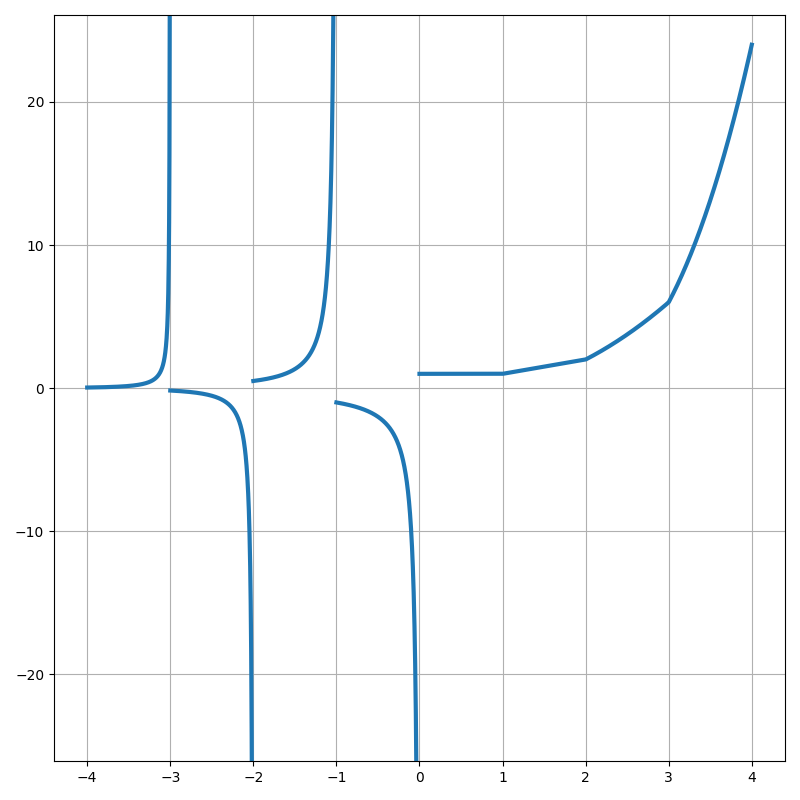
\includegraphics[width=0.8\textwidth]{UA_Section_8_4_Figure_1.png}
            \caption{\( h \) on \( [-4, 4] \)}
            \label{fig:1}
        \end{figure}
    \end{enumerate}
\end{solution}

\begin{exercise}
\label{ex:9}
    \begin{enumerate}
        \item Show that the improper integral \( \int_a^{\infty} f \) converges if and only if, for all \( \epsilon > 0 \) there exists \( M > a \) such that whenever \( d > c \geq M \) it follows that
        \[
            \abs{\int_c^d f} < \epsilon.
        \]
        (In one direction it will be useful to consider the sequence \( a_n = \int_a^{a+n} f \).)

        \item Show that if \( 0 \leq f \leq g \) and \( \int_a^{\infty} g \) converges then \( \int_a^{\infty} f \) converges.

        \item Part (a) is a Cauchy criterion, and part (b) is a comparison test. State and prove an absolute convergence test for improper integrals.
    \end{enumerate}
\end{exercise}

\begin{solution}
    \begin{enumerate}
        \item Suppose that \( \int_a^{\infty} f \) converges to some \( L \in \R \) and let \( \epsilon > 0 \) be given. There exists an \( M > a \) such that
        \[
            b \geq M \quimplies \abs{\int_a^b f - L} < \frac{\epsilon}{2}.
        \]
        It follows that for \( d > c \geq M \) we have
        \[
            \abs{\int_c^d f} = \abs{\int_a^d f - \int_a^c f - L + L} \leq \abs{\int_a^c f - L} + \abs{\int_a^d f - L} < \epsilon.
        \]
        
        Now suppose that
        \[
            \text{for all } \epsilon > 0 \text{ there exists an } M > a \text{ such that} \quad d \geq c \geq M \quimplies \abs{\int_c^d f} < \epsilon. \tag{\( * \)}
        \]
        For each \( n \in \N \) define \( a_n = \int_a^{a+n} f \). Given an \( \epsilon > 0 \), obtain an \( M \) from \( (*) \) and let \( N \in \N \) be such that \( a + N \geq M \). If \( n \geq m \geq N \), then by \( (*) \) we have
        \[
            \abs{a_n - a_m} = \abs{\int_{a+m}^{a+n} f} < \epsilon.
        \]
        Thus \( (a_n) \) is Cauchy and hence convergent, say \( \lim_{n \to \infty} a_n = L \).

        We claim that \( \int_a^{\infty} f = L \). To see this, let \( \epsilon > 0 \) be given. By \( (*) \), there is an \( M > a \) such that
        \[
            d \geq c \geq M \quimplies \abs{\int_c^d f} < \frac{\epsilon}{2}. \tag{\( \dag \)}
        \]
        Let \( N_1 \in \N \) be such that \( a + N_1 \geq M \). Since \( \lim_{n \to \infty} a_n = L \), there is an \( N_2 \in \N \) such that
        \[
            n \geq N_2 \quimplies \abs{\int_a^{a+n} f - L} < \frac{\epsilon}{2}. \tag{\( \ddag \)}
        \]
        Let \( N = \max \{ N_1, N_2 \} \) and suppose that \( b \geq a + N \). Then by \( (\dag) \) and \( (\ddag) \) we have
        \[
            \abs{\int_a^b f - L} \leq \abs{\int_a^{a+N} f - L} + \abs{\int_{a+N}^b f} < \epsilon.
        \]
        Our claim follows.

        \item The inequality \( 0 \leq f \leq g \) implies that \( 0 \leq \int_c^d f \leq \int_c^d g \) for any \( d \geq c \geq a \). Let \( \epsilon > 0 \) be given. By part (a), there is an \( M > a \) such that \( \abs{\int_c^d g} = \int_c^d g < \epsilon \) whenever \( d \geq c \geq M \). For such \( d \) and \( c \) we then have \( \abs{\int_c^d f} = \int_c^d f \leq \int_c^d g < \epsilon \). It follows from part (a) that \( \int_a^{\infty} f \) converges.

        \item We will show that if \( \int_a^{\infty} \abs{f} \) converges then so does \( \int_a^{\infty} f \). For any \( \epsilon > 0 \), part (a) implies that there is an \( M > a \) such that \( \abs{\int_c^d \abs{f}} = \int_c^d \abs{f} < \epsilon \) for any \( d \geq c \geq M \). For such \( d \) and \( c \) it follows that \( \abs{\int_c^d f} \leq \int_c^d \abs{f} < \epsilon \) and part (a) allows us to conclude that \( \int_a^{\infty} f \) converges.
    \end{enumerate}
\end{solution}

\begin{exercise}
\label{ex:10}
    \begin{enumerate}
        \item Use the properties of \( e^t \) previously discussed to show
        \[
            \int_0^{\infty} e^{-t} \, dt = 1.
        \]

        \item Show
        \makeatletter
        \tagsleft@true
        \begin{align*}
            \frac{1}{\alpha} = \int_0^{\infty} e^{-\alpha t} \, dt, \quad \text{for all } \alpha > 0. \tag{3}
        \end{align*}
        \tagsleft@false
        \makeatother
    \end{enumerate}
\end{exercise}

\begin{solution}
    \begin{enumerate}
        \item As \( \paren{ -e^{-t} }' = e^{-t} \) (chain rule and \Cref{ex:2}), the Fundamental Theorem of Calculus gives us
        \[
            \lim_{b \to \infty} \int_0^b e^{-t} \, dt = \lim_{b \to \infty} \paren{ e^0 - e^{-b} } = 1 - \lim_{b \to \infty} e^{-b} = 1,
        \]
        where we have used that \( e^0 = 1 \) (\Cref{ex:3} (b)) and that \( \lim_{b \to \infty} e^{-b} = 0 \) (\Cref{ex:5}).

        \item Similarly to part (a), this time using change of variables:
        \[
            \lim_{b \to \infty} \int_0^b e^{-\alpha t} \, dt = \lim_{b \to \infty} \alpha^{-1} \paren{ e^0 - e^{-b} } = \alpha^{-1} \paren{1 - \lim_{b \to \infty} e^{-b}} = \alpha^{-1}.
        \]
    \end{enumerate}
\end{solution}

\begin{exercise}
\label{ex:11}
    \begin{enumerate}
        \item Evaluate \( \int_0^b t e^{-\alpha t} \, dt \) using the integration-by-parts formula from \href{https://lew98.github.io/Mathematics/UA_Section_7_5_Exercises.pdf}{Exercise 7.5.6}. The result will be an expression in \( \alpha \) and \( b \).

        \item Now compute \( \int_0^{\infty} t e^{-\alpha t} \, dt \) and verify equation (4).
    \end{enumerate}
\end{exercise}

\begin{solution}
    \begin{enumerate}
        \item After applying integration-by-parts and simplifying, we find that
        \[
            \int_0^b t e^{-\alpha t} \, dt = \alpha^{-2} - \alpha^{-1} b e^{-\alpha b} - \alpha^{-2} e^{-\alpha b}.
        \]

        \item Using the expression from part (a) and \Cref{ex:5}, we see that
        \[
            \lim_{b \to \infty} \int_0^b t e^{-\alpha t} \, dt = \lim_{b \to \infty} \paren{ \alpha^{-2} - \alpha^{-1} b e^{-\alpha b} - \alpha^{-2} e^{-\alpha b} } = \alpha^{-2}.
        \]
    \end{enumerate}
\end{solution}

\begin{exercise}
\label{ex:12}
    Assume the function \( f(x, t) \) is continuous on the rectangle \( D = \{ (x, t) : a \leq x \leq b, c \leq t \leq d \} \). Explain why the function
    \[
        F(x) = \int_c^d f(x, t) \, dt
    \]
    is properly defined for all \( x \in [a, b] \).
\end{exercise}

\begin{solution}
    Here is a useful lemma.
    \begin{tcolorbox}[breakable]
        \textbf{Lemma 1.} Suppose \( f : D \to \R \) is continuous, where
        \[
            D = \{ (x, t) \in \R^2 : a \leq x \leq b, c \leq t \leq d \}.
        \]
        Then for a fixed \( x_0 \in [a, b] \), the function \( g : [c, d] \to \R \) given by \( g(t) = f(x_0, t) \) is continuous.
        \tcblower
        \textit{Proof.} Fix \( t_0 \in [c, d] \); we aim to show that \( g \) is continuous at \( t_0 \), so let \( \epsilon > 0 \) be given. By assumption \( f \) is continuous at \( (x_0, t_0) \in D \) and thus there is a \( \delta > 0 \) such that \( \abs{f(x, t) - f(x_0, t_0)} < \epsilon \) whenever \( (x, t) \in D \) and
        \[
            \norm{(x, t) - (x_0, t_0)} = \sqrt{(x - x_0)^2 - (t - t_0)^2} < \delta.
        \]
        Now suppose that \( t \in [c, d] \) is such that \( \abs{t - t_0} < \delta \). Notice that
        \[
            \norm{(x_0, t) - (x_0, t_0)} = \sqrt{(t - t_0)^2} = \abs{t - t_0} < \delta.
        \]
        It follows that
        \[
            \abs{f(x_0, t) - f(x_0, t_0)} = \abs{g(t) - g(t_0)} < \epsilon
        \]
        and hence that \( g \) is continuous at \( t_0 \), as desired. \qed
    \end{tcolorbox}
    If we fix \( x \in [a, b] \), Lemma 1 implies that \( f(x, t) \) is a continuous function of \( t \) on the interval \( [c, d] \) and hence by Theorem 7.2.9 is integrable on \( [c, d] \). Thus \( F \) is properly defined for each \( x \in [a, b] \).
\end{solution}

\begin{exercise}
\label{ex:13}
    Prove Theorem 8.4.5.
\end{exercise}

\begin{solution}
    Fix \( x_0 \in [a, b] \); we claim that \( F \) is continuous at \( x_0 \). Let \( \epsilon > 0 \) be given. Theorem 4.4.7 is easily adapted to show that \( f \) must be uniformly continuous on \( D \) and thus there exists a \( \delta > 0 \) such that
    \[
        (x, t), (y, z) \in D \text{ and } \norm{(x, t) - (y, z)} < \delta \quimplies \abs{f(x, t) - f(y, z)} < \frac{\epsilon}{d - c}.
    \]
    Suppose that \( x \in [a, b] \) is such that \( \abs{x - x_0} < \delta \). Then for any \( t \in [c, d] \) we have
    \[
        \norm{(x, t) - (x_0, t)} = \abs{x - x_0} < \delta
    \]
    and hence \( \abs{f(x, t) - f(x_0, t)} < \tfrac{\epsilon}{d - c} \). It follows that
    \[
        \abs{F(x) - F(x_0)} = \abs{\int_c^d f(x, t) - f(x_0, t) \, dt} \leq \int_c^d \abs{f(x, t) - f(x_0, t)} \, dt \leq \int_c^d \frac{\epsilon}{d - c} \, dt = \epsilon.
    \]
    Thus \( F \) is continuous on the compact set \( [a, b] \); Theorem 4.4.7 then implies that \( F \) is uniformly continuous on \( [a, b] \).
\end{solution}

\begin{exercise}
\label{ex:14}
    Finish the proof of Theorem 8.4.6.
\end{exercise}

\begin{solution}
    As \( f_x \) is continuous on the compact set \( D \), it must be uniformly continuous here. Thus there exists a \( \delta > 0 \) such that
    \[
        (z, s), (x, t) \in D \text{ and } \norm{(z, s) - (x, t)} < \delta \quimplies \abs{f_x(z, s) - f_x(x, t)} < \frac{\epsilon}{d - c}. \tag{\( * \)}
    \]
    Suppose that \( z \in [a, b] \) is such that \( 0 < \abs{z - x} < \delta \). For a given \( t \in [c, d] \), the Mean Value Theorem (Theorem 5.3.2) implies that there exists some \( y_t \) strictly between \( z \) and \( x \), so that \( \abs{y_t - x} < \abs{z - x} < \delta \), satisfying
    \[
        \frac{f(z, t) - f(x, t)}{z - x} = f_x(y_t, t).
    \]
    Notice that \( \norm{(y_t, t) - (x, t)} = \abs{y_t - x} < \delta \); it follows from \( (*) \) that \( \abs{f_x(y_t, t) - f_x(x, t)} < \tfrac{\epsilon}{d - c} \) and hence that
    \begin{multline*}
        \abs{\frac{F(z) - F(x)}{z - x} - \int_c^d f_x(x, t) \, dt} = \abs{\int_c^d \frac{f(z, t) - f(x, t)}{z - x} - f_x(x, t) \, dt} \\[2mm]
        = \abs{\int_c^d f_x(y_t, t) - f_x(x, t) \, dt} \leq \int_c^d \abs{f_x(y_t, t) - f_x(x, t)} \, dt \leq \int_c^d \frac{\epsilon}{d - c} \, dt = \epsilon.
    \end{multline*}
\end{solution}

\begin{exercise}
\label{ex:15}
    \begin{enumerate}
        \item Show that the improper integral \( \int_0^{\infty} e^{-xt} \, dt \) converges uniformly to \( 1/x \) on the set \( [1/2, \infty) \).

        \item Is the convergence uniform on \( (0, \infty) \)?
    \end{enumerate}
\end{exercise}

\begin{solution}
    \begin{enumerate}
        \item Let \( \epsilon > 0 \) be given and set \( M = \max \set{ -2 \log \paren{ \tfrac{\epsilon}{2} }, 0 } \). Then if \( d \geq M \) and \( x \geq \tfrac{1}{2} \), we have
        \[
            \abs{\frac{1}{x} - \int_0^d e^{-xt} \, dt} = \frac{e^{-xd}}{x} \leq 2 e^{-d/2} < \epsilon;
        \]
        we are using here that \( E \) is strictly increasing, which implies that its inverse function \( \log \) is also strictly increasing.

        \item The convergence is not uniform on \( (0, \infty) \). For any \( M > 0 \), we have
        \[
            \abs{\frac{1}{x} - \int_0^M e^{-xt} \, dt} = \frac{e^{-Mx}}{x}.
        \]
        Notice that \( \lim_{x \to 0^+} \tfrac{e^{-Mx}}{x} = +\infty \), since \( \lim_{x \to 0^+} e^{-Mx} = 1 \) and \( \lim_{x \to 0^+} \tfrac{1}{x} = +\infty \). Thus there is an \( x > 0 \) such that
        \[
            \abs{\frac{1}{x} - \int_0^M e^{-xt} \, dt} = \frac{e^{-Mx}}{x} \geq 1.
        \]
    \end{enumerate}
\end{solution}

\begin{exercise}
\label{ex:16}
    Prove the following analogue of the Weierstrass M-Test for improper integrals: If \( f(x, t) \) satisfies \( \abs{f(x, t)} \leq g(t) \) for all \( x \in A \) and \( \int_a^{\infty} g(t) \, dt \) converges, then \( \int_a^{\infty} f(x, t) \, dt \) converges uniformly on \( A \).
\end{exercise}

\begin{solution}
    Here is a Cauchy criterion for the uniform convergence of an improper integral, an analogue of Theorem 6.4.4.
    \begin{tcolorbox}
        \textbf{Lemma 2.} Suppose \( D = \{ (x, t) \in \R^2 : x \in A, t \geq a \} \) for some \( A \subseteq \R \) and \( a \in \R \) and we have a function \( f : D \to \R \). Then the improper integral \( \int_a^{\infty} f(x, t) \, dt \) converges uniformly to some function \( F : A \to \R \) if and only if for every \( \epsilon > 0 \) there exists an \( M \geq a \) such that
        \[
            x \in A \text{ and } c \geq b \geq M \quimplies \abs{\int_b^c f(x, t) \, dt} < \epsilon. \tag{\( * \)}
        \]
        \tcblower
        First suppose that the improper integral \( \int_a^{\infty} f(x, t) \, dt \) converges uniformly to some function \( F : A \to \R \) and let \( \epsilon > 0 \) be given. There exists an \( M \geq a \) such that
        \[
            x \in A \text{ and } b \geq M \quimplies \abs{F(x) - \int_a^b f(x, t) \, dt} < \frac{\epsilon}{2}.
        \]
        Then provided \( x \in A \) and \( c \geq b \geq M \), we have
        \begin{multline*}
            \abs{\int_b^c f(x, t) \, dt} = \abs{-F(x) + \int_a^c f(x, t) \, dt + F(x) - \int_a^b f(x, t) \, dt + F(x)} \\[2mm]
            \leq \abs{F(x) - \int_a^c f(x, t) \, dt} + \abs{F(x) - \int_a^b f(x, t) \, dt} < \epsilon.
        \end{multline*}

        Now suppose that for each \( \epsilon > 0 \) there exists an \( M \geq a \) such that \( (*) \) holds. For each \( x \in A \) we may invoke \Cref{ex:9} (a) to see that the improper integral \( \int_a^{\infty} f(x, t) \, dt \) converges; define \( F(x) \) to be this value. We claim that the improper integral \( \int_a^{\infty} f(x, t) \, dt \) converges uniformly to \( F \) on \( A \). To see this, let \( \epsilon > 0 \) be given and obtain \( M \geq a \) from \( (*) \). If \( x \in A \) and \( c \geq b \geq M \), then
        \begin{multline*}
            \abs{F(x) - \int_a^b f(x, t) \, dt} = \abs{F(x) - \int_a^c f(x, t) \, dt + \int_b^c f(x, t) \, dt} \\[2mm]
            \leq \abs{F(x) - \int_a^c f(x, t) \, dt} + \abs{\int_b^c f(x, t) \, dt} < \abs{F(x) - \int_a^c f(x, t) \, dt} + \epsilon.
        \end{multline*}
        Notice that this inequality holds for all \( c \in [b, \infty) \). Since \( \lim_{c \to \infty} g(c) = L \) implies \( \lim_{c \to \infty} \abs{g(c)} = \abs{L} \), we can take the limit as \( c \to \infty \) on both sides of the above inequality to obtain
        \begin{multline*}
            \lim_{c \to \infty} \abs{F(x) - \int_a^b f(x, t) \, dt} = \abs{F(x) - \int_a^b f(x, t) \, dt} \\[2mm]
            \leq \lim_{c \to \infty} \paren{ \abs{F(x) - \int_a^c f(x, t) \, dt} + \epsilon } = \abs{F(x) - \lim_{c \to \infty} \int_a^c f(x, t) \, dt} + \epsilon = \epsilon,
        \end{multline*}
        i.e.\ \( \abs{F(x) - \int_a^b f(x, t) \, dt} \leq \epsilon \). We may conclude that the improper integral \( \int_a^{\infty} f(x, t) \, dt \) converges uniformly to \( F \) on \( A \). \qed
    \end{tcolorbox}
    Returning to the exercise, let \( \epsilon > 0 \) be given. By \Cref{ex:9} (a) there exists an \( M \geq a \) such that
    \[
        x \in A \text{ and } c \geq b \geq M \quimplies \int_b^c g(t) \, dt < \epsilon.
    \]
    It follows that for \( x \in A \) and \( c \geq b \geq M \) we have
    \[
        \abs{\int_b^c f(x, t) \, dt} \leq \int_b^c \abs{f(x, t)} \, dt \leq \int_b^c g(t) \, dt < \epsilon.  
    \]
    Lemma 2 allows us to conclude that the improper integral \( \int_a^{\infty} f(x, t) \, dt \) converges uniformly on \( A \).
\end{solution}

\begin{exercise}
\label{ex:17}
    Prove Theorem 8.4.8.
\end{exercise}

\begin{solution}
    For each \( n \in \N \), define \( F_n : [a, b] \to \R \) by
    \[
        F_n(x) = \int_c^{c+n} f(x, t) \, dt.
    \]
    By assumption \( f \) is continuous on \( [a, b] \times [c, c+n] \) and so by Theorem 8.4.5 each \( F_n \) is uniformly continuous on \( [a, b] \). As noted in the textbook, \( F_n \) converges to \( F \) uniformly on \( [a, b] \). We may use \href{https://lew98.github.io/Mathematics/UA_Section_6_2_Exercises.pdf}{Exercise 6.2.6 (a)} to conclude that \( F \) is uniformly continuous on \( [a, b] \).
\end{solution}

\begin{exercise}
\label{ex:18}
    Prove Theorem 8.4.9.
\end{exercise}

\begin{solution}
    For each \( n \in \N \), define \( F_n : [a, b] \to \R \) and \( G : [a, b] \to \R \) by
    \[
        F_n(x) = \int_c^{c+n} f(x, t) \, dt \quand G(x) = \int_c^{\infty} f_x(x, t) \, dt.
    \]
    By Theorem 8.4.6 we have \( F_n'(x) = \int_c^{c+n} f_x(x, t) \, dt \) and hence by assumption \( F_n' \to G \) uniformly on \( [a, b] \). Notice that our hypotheses imply
    \[
        \lim_{n \to \infty} F_n(a) = \lim_{d \to \infty} \int_c^d f(a, t) \, dt = F(a).
    \]
    We may now use Theorem 6.3.3 to see that \( F_n \to F \) uniformly on \( [a, b] \) and furthermore that
    \[
        F'(x) = G(x) = \int_c^{\infty} f_x(x, t) \, dt.
    \]
\end{solution}

\begin{exercise}
\label{ex:19}
    \begin{enumerate}
        \item Although we verified it directly, show how to use the theorems in this section to give a second justification for the formula
        \[
            \frac{1}{\alpha^2} = \int_0^{\infty} t e^{-\alpha t} \, dt, \quad \text{for all } \alpha > 0.
        \]

        \item Now derive the formula
        \makeatletter
        \tagsleft@true
        \begin{align*}
            \frac{n!}{\alpha^{n+1}} = \int_0^{\infty} t^n e^{-\alpha t} \, dt, \quad \text{for all } \alpha > 0. \tag{8}
        \end{align*}
        \tagsleft@false
        \makeatother
    \end{enumerate}
\end{exercise}

\begin{solution}
    We will need the following results about continuous functions, the proofs of which are straightforward and hence, for the sake of brevity, omitted.
    \begin{tcolorbox}
        \textbf{Lemma 3.} Suppose that \( f, g : D \to \R \), where \( D \subseteq \R^2 \), are continuous functions.
        \begin{enumerate}[label=(\roman*)]
            \item The function \( (x, y) \mapsto f(x, y) g(x, y) \) is continuous on \( D \).

            \item The function \( (x, y) \mapsto k f(x, y) \), for some \( k \in \R \), is continuous on \( D \).

            \item If \( h : A \to \R \) is continuous, where \( A \subseteq f(D) \subseteq \R \), then the function \( (x, y) \mapsto h(f(x, y)) \) is continuous on \( D \).
        \end{enumerate}
    \end{tcolorbox}


    \begin{enumerate}
        \item Define \( f : \R^2 \to \R \) by \( f(\alpha, t) = e^{-\alpha t} \). It is easy to verify that the projections \( (\alpha, t) \mapsto \alpha \) and \( (\alpha, t) \mapsto t \) are continuous on all of \( \R^2 \); it follows from this fact and Lemma 3 that \( f \) is continuous on all of \( \R^2 \). Notice that \( f_{\alpha}(\alpha, t) = -t e^{-\alpha t} \) exists for all \( (\alpha, t) \in \R^2 \); we can argue as before to see that \( f_{\alpha} \) is continuous on all of \( \R^2 \).

        Let \( 0 < a < b \) be arbitrary and define \( D = [a, b] \times [0, \infty) \); the previous paragraph shows that \( f \) and \( f_{\alpha} \) are continuous on \( D \). Furthermore, by \Cref{ex:10} (b), the function \( F : [a, b] \to \R \) given by
        \[
            F(\alpha) = \int_0^{\infty} f(\alpha, t) \, dt
        \]
        is well-defined and satisfies \( F(\alpha) = \tfrac{1}{\alpha} \), so that \( F'(\alpha) = -\tfrac{1}{\alpha^2} \).

        Now we claim that the improper integral
        \[
            \int_0^{\infty} f_{\alpha}(\alpha, t) \, dt = \int_0^{\infty} -t e^{-\alpha t} \, dt
        \]
        converges uniformly on \( [a, b] \). Notice that
        \[
            \abs{f_{\alpha}(\alpha, t)} = t e^{-\alpha t} \leq t e^{-at}
        \]
        for each \( \alpha \in [a, b] \) and \( t \geq 0 \). Hence, by \Cref{ex:16}, it will suffice to show that the improper integral \( \int_0^{\infty} t e^{-at} \, dt \) converges. (Of course, we can show directly using integration-by-parts that it converges to \( \tfrac{1}{a^2} \), as we did in \Cref{ex:11}, making this exercise redundant. However, since presumably the purpose of this exercise is to practice using the theorems and results of this section, we will proceed differently.) By \Cref{ex:5} we have \( \lim_{t \to \infty} t e^{-at/2} = 0 \) and so there exists an \( M > 0 \) such that
        \[
            t e^{-at/2} \leq 1 \quiff t e^{-at} \leq e^{-at/2}
        \]
        for all \( t > M \). Since \( t \mapsto t e^{-at} \) is continuous on \( [0, M] \) it must be bounded here, say by \( L \geq 0 \). Thus if we define \( g : [0, \infty) \to \R \) by
        \[
            g(t) = \begin{cases}
                L & \text{if } 0 \leq t \leq M, \\
                e^{-at/2} & \text{if } t > M,
            \end{cases}
        \]
        then \( 0 \leq t e^{-at} \leq g(t) \) for all \( t \geq 0 \). A direct calculation shows that
        \[
            \int_0^{\infty} g(t) \, dt = LM + \frac{2 e^{-aM/2}}{a}
        \]
        and hence by \Cref{ex:9} (b) the improper integral \( \int_0^{\infty} t e^{-at} \, dt \) also converges. We may now apply \Cref{ex:16} to see that the improper integral \( \int_0^{\infty} f_{\alpha}(\alpha, t) \, dt \) converges uniformly on \( [a, b] \).

        We have now satisfied all the hypotheses of Theorem 8.4.9. Applying this theorem shows that
        \[
            \frac{1}{\alpha^2} = -F'(\alpha) = -\int_0^{\infty} f_{\alpha}(\alpha, t) \, dt = \int_0^{\infty} t e^{-\alpha t} \, dt
        \]
        for all \( \alpha \in [a, b] \). Since \( 0 < a < b \) were arbitrary, we may conclude that this formula holds for all \( \alpha > 0 \).

        \item Let's prove this by induction; the case \( n = 0 \) was handled in \Cref{ex:10} (b) and the case \( n = 1 \) was handled in \Cref{ex:11} (and also part (a) of this exercise). Suppose that the result is true for some \( n \geq 0 \). Let \( \alpha > 0 \) be given and note that, for any \( b > 0 \), integration-by-parts gives us
        \[
            \int_0^b t^{n+1} e^{-\alpha t} \, dt = -b^{n+1} e^{-\alpha b} + \frac{n + 1}{\alpha} \int_0^b t^n e^{-\alpha t} \, dt.
        \]
        \Cref{ex:5} shows that \( \lim_{b \to \infty} b^{n+1} e^{-\alpha b} = 0 \) and our induction hypothesis ensures that \( \int_0^{\infty} t^n e^{-\alpha t} \, dt = \frac{n!}{\alpha^{n+1}} \); it follows that
        \[
            \int_0^{\infty} t^{n+1} e^{-\alpha t} \, dt = \frac{n + 1}{\alpha} \cdot \frac{n!}{\alpha^{n+1}} = \frac{(n + 1)!}{\alpha^{n+2}}.
        \]
        This completes the induction step and the proof.
    \end{enumerate}
\end{solution}

\begin{exercise}
\label{ex:20}
    \begin{enumerate}
        \item Show that \( x! \) is an infinitely differentiable function on \( (0, \infty) \) and produce a formula for the \( n \)\ts{th} derivative. In particular show that \( (x!)'' > 0 \).

        \item Use the integration-by-parts formula employed earlier to show that \( x! \) satisfies the functional equation
        \[
            (x + 1)! = (x + 1)x!.
        \]
    \end{enumerate}
\end{exercise}

\begin{solution}
    The definition \( x! = \int_0^{\infty} t^x e^{-t} \, dt \) involves an improper integral as defined in Definition 8.4.3. This definition requires the integrand \( t^x e^{-t} \) to be defined on \( [0, \infty) \), but in fact it is undefined for \( t = 0 \). I am going to ignore this issue.
    \begin{enumerate}
        \item For \( n \in \N \), let us denote the \( n \)\ts{th} derivative of \( x! \) by \( (x!)^{(n)} \). We will prove by induction that
        \[
            (x!)^{(n)} = \int_0^{\infty} \paren{ \log t }^{n} t^x e^{-t} \, dt
        \]
        for \( x > 0 \). For the base case \( n = 1 \), first observe that
        \[
            \frac{d}{dx} \paren{ t^x e^{-t} } = (\log t) t^x e^{-t}.
        \]
        Let \( 0 < a < b \) be arbitrary; we claim that the improper integral \( \int_0^{\infty} (\log t) t^x e^{-t} \, dt \) converges uniformly on \( [a, b] \). To see this, note that
        \[
            \abs{(\log t) t^x e^{-t}} = (\log t) t^x e^{-t} \leq t^{x + 1} e^{-t} \leq t^{b + 1} e^{-t}
        \]
        for \( x \in [a, b] \) and \( t \geq 1 \). Note further that
        \[
            \abs{(\log t) t^x e^{-t}} = \abs{\log t} t^x e^{-t} \leq \abs{\log t} t^b
        \]
        for \( x \in [a, b] \) and \( 0 < t < 1 \). Since
        \[
            \lim_{t \to 0^+} \abs{\log t} t^b = 0,
        \]
        which can be seen using L'Hôpital's rule, there exists an \( M > 0 \) such that \( \abs{\log t} t^b \leq M \) for all \( x \in [a, b] \) and \( 0 < t < 1 \). Thus, if we define
        \[
            g(t) = \begin{cases}
                M & \text{if } 0 < t < 1, \\
                t^{b + 1} e^{-t} & \text{if } t \geq 1,
            \end{cases}
        \]
        then \( \abs{(\log t) t^x e^{-t}} \leq g(t) \). It is straightforward to show that \( \int_0^{\infty} g(t) \, dt \) converges and so it follows from \Cref{ex:16} that \( \int_0^{\infty} (\log t) t^x e^{-t} \, dt \) converges uniformly on \( [a, b] \). We can now use Theorem 8.4.9 to see that
        \[
            (x!)' = \int_0^{\infty} (\log t) t^x e^{-t} \, dt
        \]
        for \( x \in [a, b] \). Since \( 0 < a < b \) were arbitrary, we see that this formula holds for all \( x > 0 \).

        The induction step is essentially identical to the base case; note that
        \[
            \frac{d}{dx} \paren{ (\log t)^n t^x e^{-t} } = (\log t)^{n+1} t^x e^{-t}.
        \]
        For arbitrary \( 0 < a < b \), we can again bound \( \abs{ (\log t)^{n+1} t^x e^{-t} } \) by
        \[
            g(t) = \begin{cases}
                M & \text{if } 0 < t < 1, \\
                t^{b + n + 1} e^{-t} & \text{if } t \geq 1,
            \end{cases}
        \]
        where \( M > 0 \) is some bound on \( \abs{(\log t)^{n+1} t^x e^{-t}} \) for \( x \in [a, b] \) and \( 0 < t < 1 \); the existence of this \( M \) follows since
        \[
            \lim_{t \to 0^+} \abs{\log t}^{n+1} t^b = 0,
        \]
        which can be seen by repeated applications of L'Hôpital's rule. Then since \( \int_0^{\infty} g(t) \, dt \) converges, \Cref{ex:16} implies that the improper integral \( \int_0^{\infty} (\log t)^{n+1} t^x e^{-t} \, dt \) converges uniformly on \( [a, b] \) and hence by Theorem 8.4.9 we have
        \[
            (x!)^{(n+1)} = \frac{d}{dx} (x!)^{(n)} = \int_0^{\infty} (\log t)^{n+1} t^x e^{-t} \, dt
        \]
        for all \( x \in [a, b] \). Since \( 0 < a < b \) were arbitrary, the formula holds for all \( x > 0 \). This completes the induction step and the proof.

        In particular, we have
        \[
            (x!)'' = \int_0^{\infty} (\log t)^2 t^x e^{-t} \, dt.
        \]
        The integrand \( (\log t)^2 t^x e^{-t} \) is strictly positive for all \( x > 0 \) and \( t > 1 \), whence \( (x!)'' > 0 \).

        \item For any \( b > 0 \), integration-by-parts gives
        \[
            \int_0^b t^{x+1} e^{-t} \, dt = -b^{x+1} e^{-b} + (x+1) \int_0^b t^x e^{-t} \, dt,
        \]
        which converges to \( (x + 1) x! \) as \( b \to \infty \).
    \end{enumerate}
\end{solution}

\begin{exercise}
\label{ex:21}
    \begin{enumerate}
        \item Use the convexity of \( \log (f(x)) \) and the three intervals \( [n - 1, n], [n, n + x], \) and \( [n, n + 1] \) to show
        \[
            x \log (n) \leq \log (f(n + x)) - \log (n!) \leq x \log (n + 1).
        \]

        \item Show \( \log (f(n + x)) = \log (f(x)) + \log ((x + 1)(x + 2) \cdots (x + n)) \).

        \item Now establish that
        \[
            0 \leq \log (f(x)) - \log \paren{ \frac{n^x n!}{(x + 1)(x + 2) \cdots (x + n)} } \leq x \log \paren{ 1 + \frac{1}{n} }.
        \]

        \item Conclude that
        \[
            f(x) = \lim_{n \to \infty} \frac{n^x n!}{(x + 1)(x + 2) \cdots (x + n)}, \quad \text{for all } x \in (0, 1].
        \]

        \item Finally, show that the conclusion in (d) holds for all \( x \geq 0 \).
    \end{enumerate}
\end{exercise}

\begin{solution}
    \begin{enumerate}
        \item First consider the intervals \( [n - 1, n] \) and \( [n, n + x] \). Using the fact about convex functions mentioned previously in the textbook, we find the inequality
        \[
            \log(f(n)) - \log(f(n-1)) \leq \frac{\log(f(n + x)) - \log(f(n))}{x}.
        \]
        Since \( f(n) = n! \) and \( \log(a) - \log(b) = \log \paren{ \tfrac{a}{b} } \), we have
        \[
            \log(f(n)) - \log(f(n-1)) = \log(n!) - \log((n-1)!) = \log \paren{ \frac{n!}{(n - 1)!} } = \log(n).
        \]
        Thus we obtain \( x \log(n) \leq \log(f(n + x)) - \log(n!) \). A similar argument with the intervals \( [n, n + x] \) and \( [n, n + 1] \) (remembering that \( x \leq 1 \)) gives us the other desired inequality.

        \item Property (ii) implies that
        \[
            f(x + n) = f(x)(x + 1)(x + 2) \cdots (x + n).
        \]
        Now we can use that \( \log(ab) = \log(a) + \log(b) \) to obtain the desired equality.

        \item Part (a) gives us
        \[
            0 \leq \log (f(n + x)) - \log (n!) - x \log (n) \leq x \log (n + 1) - x \log (n).
        \]
        Part (b) and the usual properties of logarithms imply that
        \begin{multline*}
            \log (f(n + x)) - \log (n!) - x \log (n) = \log (f(x)) + \log ((x+1) \cdots (x+n)) - \log(n^x n!) \\[2mm]
            = \log (f(x)) - \log \paren{ \frac{n^x n!}{(x + 1) \cdots (x + n)} }.
        \end{multline*}
        Similarly,
        \[
            x \log (n + 1) - x \log (n) = x \paren{ \log (n + 1) - \log (n) } = x \log \paren{ \frac{n + 1}{n} } = x \log \paren{ 1 + \frac{1}{n} }.
        \]
        Combining these gives the desired result.

        \item Since \( \log \paren{ 1 + \tfrac{1}{n} } \to 0 \), the Squeeze Theorem and part (c) imply that
        \[
            \log(f(x)) = \lim_{n \to \infty} a_n \quad \text{where } a_n = \log \paren{ \frac{n^x n!}{(x + 1)(x + 2) \cdots (x + n)} }
        \]
        for each \( x \in (0, 1] \). Since the exponential function is continuous everywhere, the above equation implies that
        \[
            f(x) = e^{\lim a_n} = \lim_{n \to \infty} e^{a_n} = \lim_{n \to \infty} \frac{n^x n!}{(x + 1)(x + 2) \cdots (x + n)}
        \]
        for each \( x \in (0, 1] \).

        \item For \( x = 0 \) we have
        \[
            \frac{n^x n!}{(x + 1)(x + 2) \cdots (x + n)} = \frac{n^0 n!}{n!} = 1 = f(0).
        \]
        For \( x > 0 \), let \( m \in \N \) be such that \( x \in (0, m] \). By repeating our previous argument with the intervals \( [n - 1, n], [n, n + x], \) and \( [n, n + m] \), we arrive at the inequality
        \[
            0 \leq \log(f(x)) - \log \paren{ \frac{n^x n!}{(x + 1)(x + 2) \cdots (x + n)} } \leq \frac{x}{m} \log \paren{ \frac{(n + m)!}{n! n^m} }.
        \]
        Notice that
        \[
            \frac{(n + m)!}{n! n^m} = \frac{(n + m)(n + m - 1) \cdots (n + 1)}{n^m} = \paren{ 1 + \frac{m}{n} } \paren{ 1 + \frac{m - 1}{n} } \cdots \paren{ 1 + \frac{1}{n} }.
        \]
        Since each of the \( m \) terms in parentheses on the right-hand side converges to 1, we see that \( \lim_{n \to \infty} \tfrac{(n + m)!}{n! n^m} = 1 \) and thus
        \[
            \lim_{n \to \infty} \frac{x}{m} \log \paren{ \frac{(n + m)!}{n! n^m} } = 0.
        \]
        We can now argue as in part (d) using the Squeeze Theorem to see that
        \[
            f(x) = \lim_{n \to \infty} \frac{n^x n!}{(x + 1)(x + 2) \cdots (x + n)}.
        \]
    \end{enumerate}
\end{solution}

\begin{exercise}
\label{ex:22}
    \begin{enumerate}
        \item Where does \( g(x) = \frac{x}{x!(-x)!} \) equal zero?
        What other familiar function has the same set of roots?

        \item The function \( e^{-x^2} \) provides the raw material for the all-important Gaussian bell curve from probability, where it is known that \( \int_{-\infty}^{\infty} e^{-x^2} \, dx = \sqrt{\pi} \). Use this fact (and some standard integration techniques) to evaluate \( (1/2)! \).

        \item Now use (a) and (b) to conjecture a striking relationship between the factorial function and a well-known function from trigonometry.
    \end{enumerate}
\end{exercise}

\begin{solution}
    \begin{enumerate}
        \item We are taking \( \tfrac{1}{x!} \) to be zero when \( x = -1, -2, -3, \ldots \) and thus \( g \) is zero at each integer. The function \( \sin(\pi x) \) has the same set of roots.

        \item For any \( b > 0 \), standard integration techniques give us
        \[
            \int_0^b \sqrt{t} e^{-t} \, dt = \int_0^{\sqrt{b}} 2 u^2 e^{-u^2} \, du = - \sqrt{b} e^{-b} + \int_0^{\sqrt{b}} e^{-u^2} \, du,
        \]
        which, given that \( \int_{-\infty}^{\infty} e^{-u^2} \, du = \sqrt{\pi} \), converges to \( \tfrac{\sqrt{\pi}}{2} \) as \( b \to \infty \). Thus
        \[
            (1/2)! = \int_0^{\infty} \sqrt{t} e^{-t} \, dt = \frac{\sqrt{\pi}}{2}.
        \]

        \item We conjecture that \( \tfrac{x}{x!(-x)!} = k \sin(\pi x) \) for some \( k \in \R \). Taking \( x = \tfrac{1}{2} \) gives us \( k = \frac{1/2}{(1/2)!(-1/2)!} \). Using part (b) and the identity \( (1/2)! = (1/2)(-1/2)! \), we find that \( k = \tfrac{1}{\pi} \).
    \end{enumerate}
\end{solution}

\begin{exercise}
\label{ex:23}
    As a parting shot, use the value for \( (1/2)! \) and the Gauss product formula in equation (9) to derive the famous product formula for \( \pi \) discovered by John Wallis in the 1650s:
    \[
        \frac{\pi}{2} = \lim_{n \to \infty} \paren{ \frac{2 \cdot 2}{1 \cdot 3} } \paren{ \frac{4 \cdot 4}{3 \cdot 5} } \paren{ \frac{6 \cdot 6}{5 \cdot 7} } \cdots \paren{ \frac{2n \cdot 2n}{(2n - 1)(2n + 1)} }.
    \]
\end{exercise}

\begin{solution}
    Taking \( x = 1/2 \) in equation (9) gives
    \[
        (1/2)! = \frac{\sqrt{\pi}}{2} = \lim_{n \to \infty} \frac{\sqrt{n} (n!)}{\paren{ \tfrac{3}{2} } \paren{ \tfrac{5}{2} } \cdots \paren{ \tfrac{2n+1}{2} }} = \lim_{n \to \infty} \frac{\sqrt{n} 2^n (n!)}{3 \cdot 5 \cdots (2n + 1)} = \lim_{n \to \infty} \frac{\sqrt{n} \cdot 2 \cdot 4 \cdots (2n)}{3 \cdot 5 \cdots (2n + 1)}.
    \]
    Squaring both sides of this equality, using the continuity of \( x \mapsto x^2 \), and multiplying through by 2 gives us
    \begin{multline*}
        \frac{\pi}{2} = \lim_{n \to \infty} \paren{ \frac{2 \cdot 2}{3 \cdot 3} } \paren{ \frac{4 \cdot 4}{5 \cdot 5} } \cdots \paren{ \frac{2n \cdot 2n}{(2n + 1)(2n + 1)} } (2n) \\[2mm]
        = \lim_{n \to \infty} \paren{ \frac{2 \cdot 2}{1 \cdot 3} } \paren{ \frac{4 \cdot 4}{3 \cdot 5} } \cdots \paren{ \frac{2n \cdot 2n}{(2n - 1)(2n + 1)} } \paren{ \frac{2n}{2n + 1} }.
    \end{multline*}
    Since \( \lim_{n \to \infty} \tfrac{2n}{2n + 1} = 1 \), it must be the case that
    \[
        \frac{\pi}{2} = \lim_{n \to \infty} \paren{ \frac{2 \cdot 2}{1 \cdot 3} } \paren{ \frac{4 \cdot 4}{3 \cdot 5} } \paren{ \frac{6 \cdot 6}{5 \cdot 7} } \cdots \paren{ \frac{2n \cdot 2n}{(2n - 1)(2n + 1)} }.
    \]
\end{solution}

\noindent \hrulefill

\noindent \hypertarget{ua}{\textcolor{blue}{[UA]} Abbott, S. (2015) \textit{Understanding Analysis.} 2\ts{nd} edition.}

\end{document}